% Methods
In this chapter, a description of event selection is given, as well as definitions of
key physical variables and how they are used to select events. Then, a procedure regarding
how the signal sample is manipulated to produce a high statistics off-shell tail is described.
Finally, the binning of variables used to obtain the results is determined and defined.

\section{Event selection and physical variables}
% \begin{itemize}
%     \item Description of homebrew event variables and their physical significance
%     \item DJJ\_VBF prescription
% \end{itemize}
Proton bunches cross each at a rate of about \SI{400}{\mega\hertz} in the beam line of
the LHC, naturally, not all of these crossings are recorded due to both technical
limitation of the electronics as well as the fact that the vast majority of these
crossings don't produce inelastic collision that is energetic enough to be interesting to us.

After the selection of Level 1 (L1) trigger and the higher level trigger (HLT), less than 1000
events per second are permanently recorded and would go to off-line, full reconstruction. Among these,
we only select the ones that passes certain triggers.
\todo[inline]{give a correct account for what trigger is used for 2018
TriggerHelpers::kDoubleMu, TriggerHelpers::kDoubleEle, Trigger Help.cc
TriggerHelpers::kSingleMu, TriggerHelpers::kSingleEle range pt
}

The jets are all AK4 jets unless mentioned otherwise. We shall also define a few of the
uncommon variables in the list, and will give a few physical motivation in the next few
paragraphs.

After selecting mandating passing certain triggers, we make a base line cut in the variables
based on more delicate physics reason, the list of base line cuts is as below:
\begin{itemize}
    \item No ak4-jet b-tagged jet
    \item Both leptons have $p_\mathrm{T} > \SI{25}{\giga\electronvolt}$
    \item $\abs{\Delta\phi_{\ell\ell\_\met}} > 1.0$
    \item $\abs{\Delta\phi_{\ell\ell\mathrm{Jets}\_\met}} > 2.5$
    \item $\abs{m_{\ell\ell} - 91.2\gev} < 15\gev$:
        the signal process consists of $\mathrm{Z}\rightarrow{}\ell\ell$, we
        require the di-lepton system has a mass that is consistent within the Z mass peak.
    \item $p_\mathrm{T}^{\ell\ell} > 55\gev$: 
        the Drell–Yan (DY) process creates a lot of backgrounds events, but their di-leptons
        go back-to-back with expected value of this variable close to 0.
    \item $\met > 125\gev$:
        the signal process creates true $\met$ with neutrinos, this cut also reduce bkg such
        as DY.
    \item $\min{\abs{ \Delta\phi_{\mathrm{j}\_\met}}} > 0.25$
    %eta muon < 2.4
    %eta electron < 2.5
    % \item $p_\mathrm{T}^{\ell\ell} > 55\gev$
\end{itemize}
% \todo[inline]{define the uncommon ones and give account for the choice}
% \missingfigure{Show how much backgrounds are gone for maybe 2 samples}

A lot of the cuts are related to angles between various physical objects presented in the
reconstruction. The reason is simple: the signal events, where Higgs goes to ZZ and one Z
goes to 2 charged lepton the other goes to 2 neutrinos, ideally would have the two Z's 
`back-to-back' in Higgs' rest frame leading to a large angel in the transverse plane. (
assuming the $\met$ mainly comes from the two neutrinos, of course)

Furthermore, in background events which do not mandate this kinematic feature, the
correlation in the directions of $\met$ and of observable physical objects is weaker.

To use this kinematic feature to increase signal to background ratio, we define 
$\abs{\Delta\phi_{\ell\ell\_\met}}$ as the azimuthal angel (perpendicular to 
the beam line) between the di-lepton system and the transverse missing energy. In the
signal events that produce 0 jet, this variable should be $\pi$. The cut is lowered to $1.0$ 
due to the finding that in the (not so rare) case where there are jet(s) recoiling against
the ZZ system, the variable dips quite low.

This leads to the next variable on the list $\abs{\Delta\phi_{\ell\ell\mathrm{Jets}\_\met}}$, which
is almost the same except that we add all jets' momentum into the di-lepton system to account
for the events that have produced jets, which in turn would cause the angel be lower in such
a multi-body final states.

Finally, $\min{\abs{ \Delta\phi_{\mathrm{j}\_\met}}}$ is the minimum azimuthal angel difference between
any of the jet (that passes cuts) and the $\met$, it exist because jets are as mentioned, one of the 
most difficult physical objects measure, they often create so-called instrumental $\met$ due to jet
mismeasurements and it can be quite large in magnitude. However, such mismeasurements often yields large
$\met$ in the direction of the original jet. This cuts requires angular separation since in signal process,
the jet recoils against ZZ system.
\newpage\phantom{blabla}

\section{Signal simulation reweighting}
\begin{itemize}
    \item Physics of Higgs signal sample (the weight, ME)
    \item the need for pieceing together samples with different LHE Mass
    \item results (also see appendix A)
\end{itemize}

\begin{figure}[htb]
\begin{center}
\subfloat[]      {
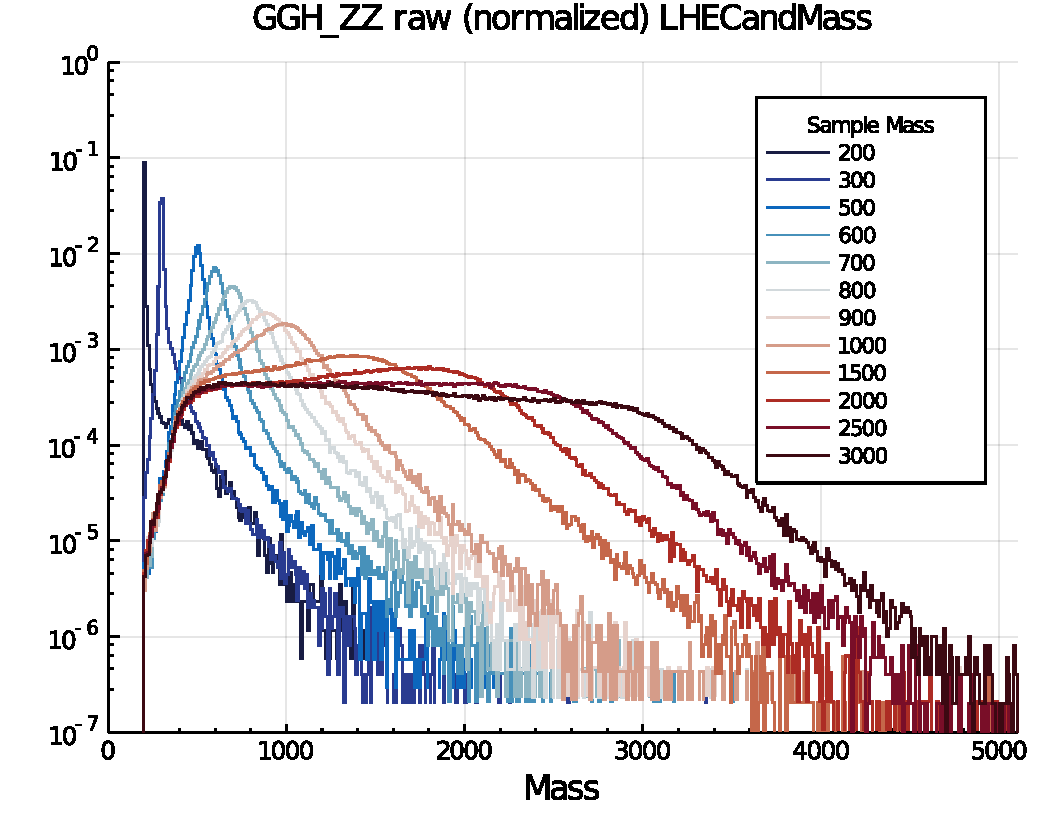
\includegraphics[width=.45\linewidth]{fig/LHE_Raw.pdf}
}\quad
\subfloat[]      {
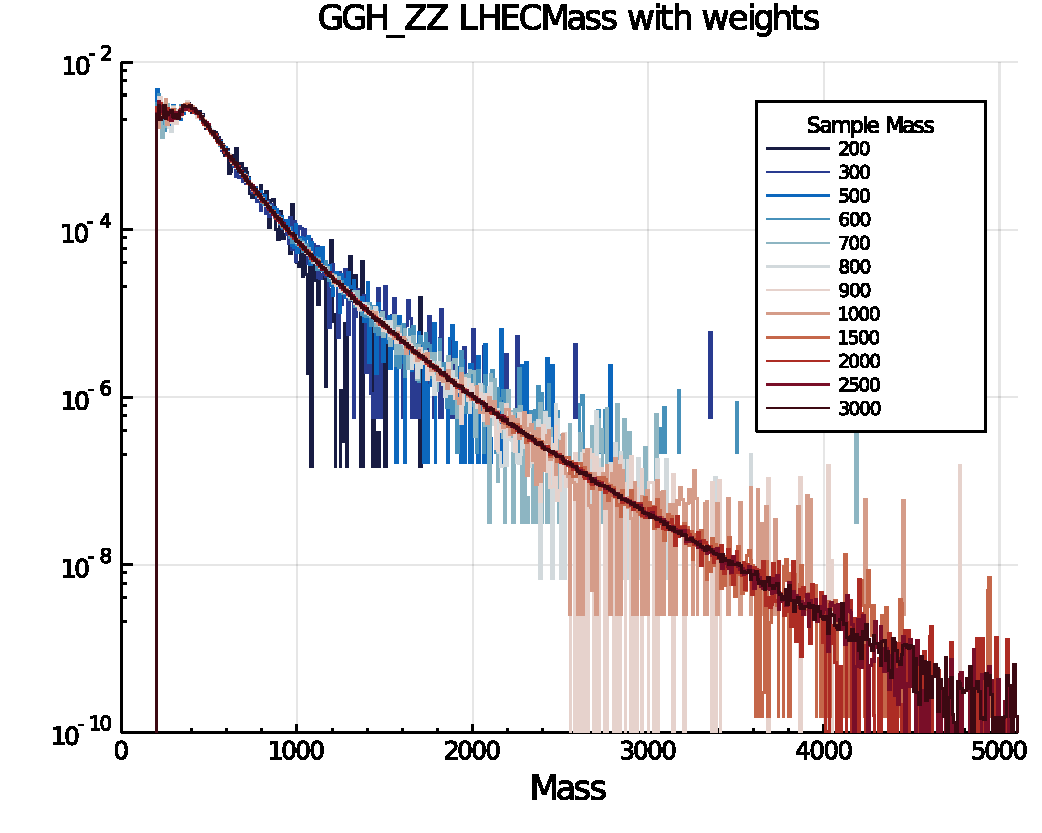
\includegraphics[width=.45\linewidth]{fig/LHE_PUME_wgts.pdf}
}\\
\subfloat[]      {
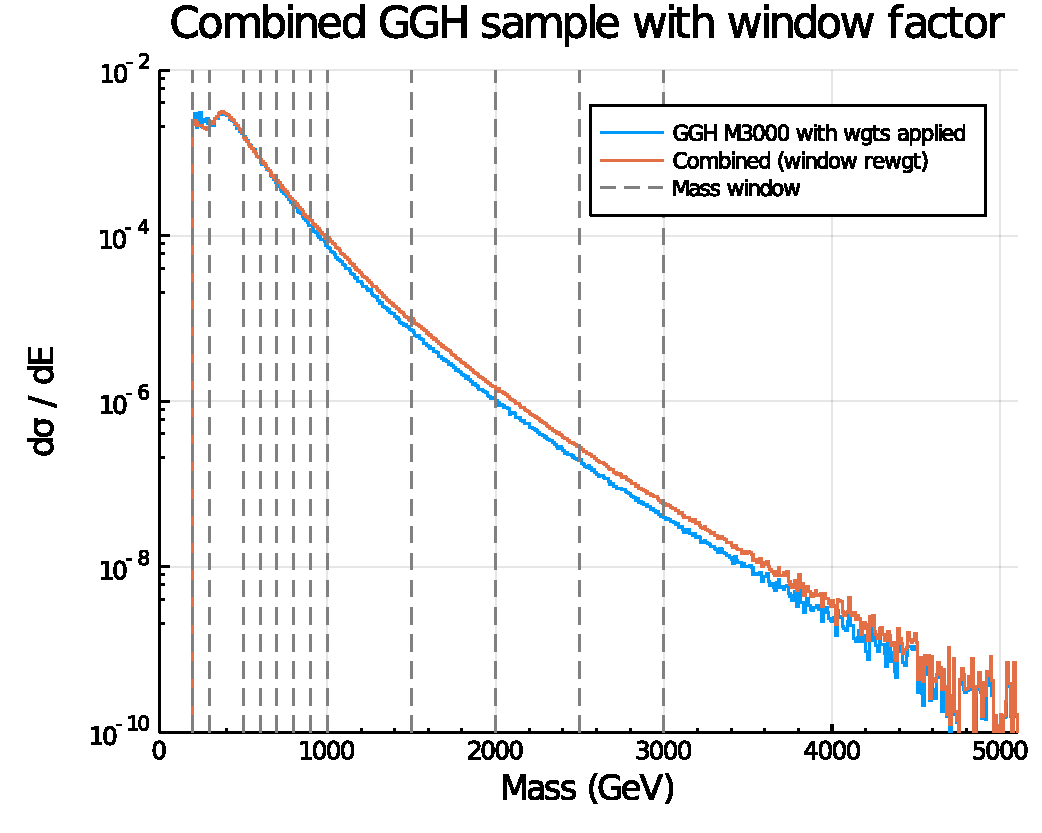
\includegraphics[width=.45\linewidth]{fig/LHC_compare_windowwgt.pdf}
}\quad
\subfloat[]      {
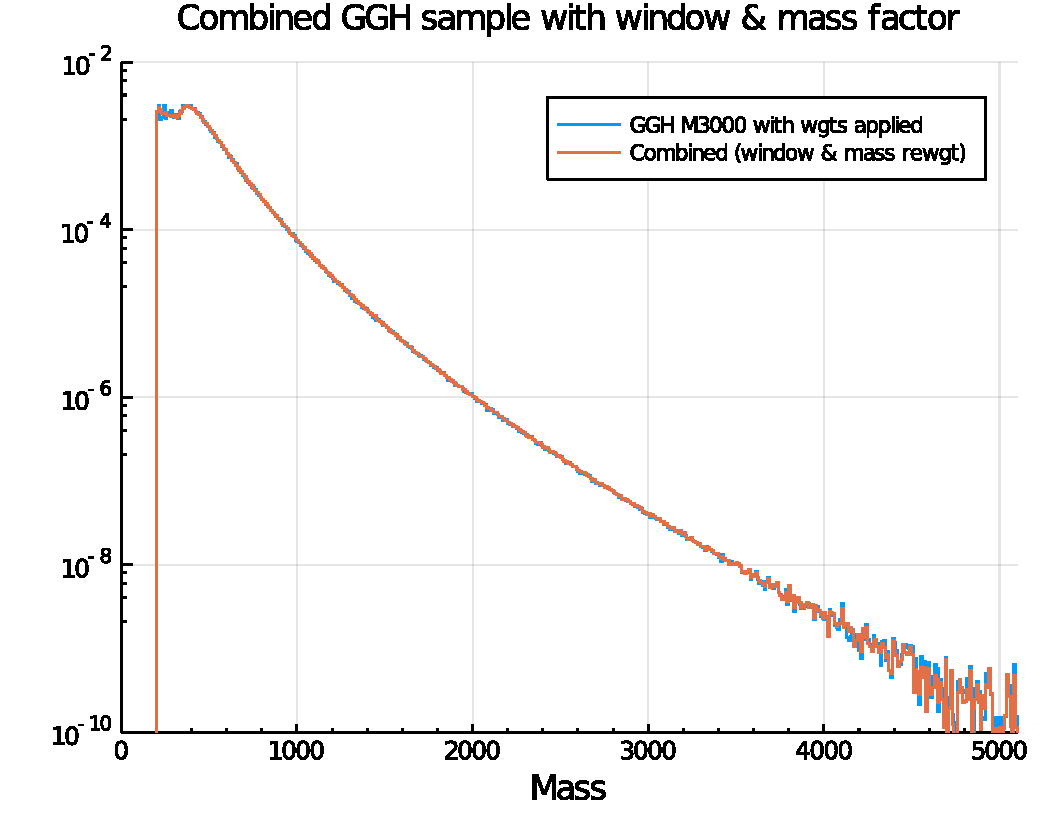
\includegraphics[width=.45\linewidth]{fig/LHC_compare_bothwgt.pdf}
}
\end{center}
\caption{TO BE ADDED}
\label{fig:LHE_rewgt}
\end{figure}
\todo[inline]{describe these steps}

\begin{figure}[htb]
\begin{center}
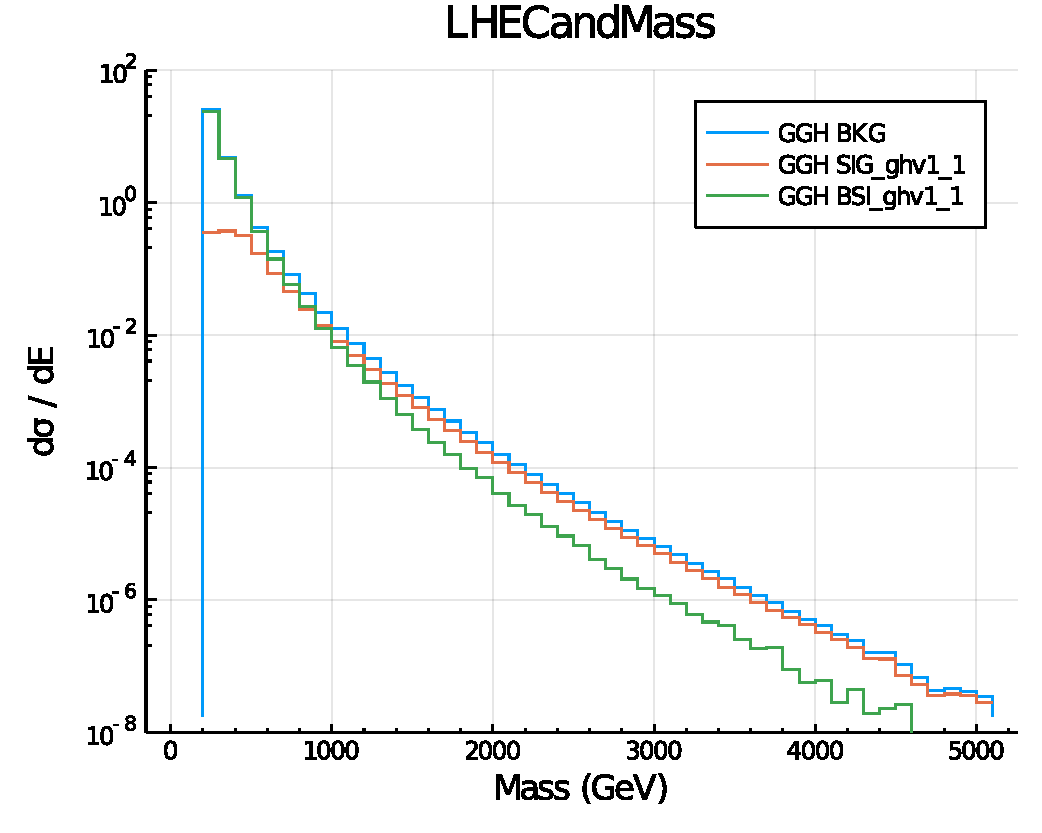
\includegraphics[width=.70\linewidth]{fig/LHE_integral_difference.pdf}
\end{center}
\caption{TO BE ADDED}
\label{fig:bsi_sig_bkg_compare}
\end{figure}
\newpage\phantom{blabla}


\section{Strategy in variable selection and binning}
\begin{figure}[htb]
\begin{center}
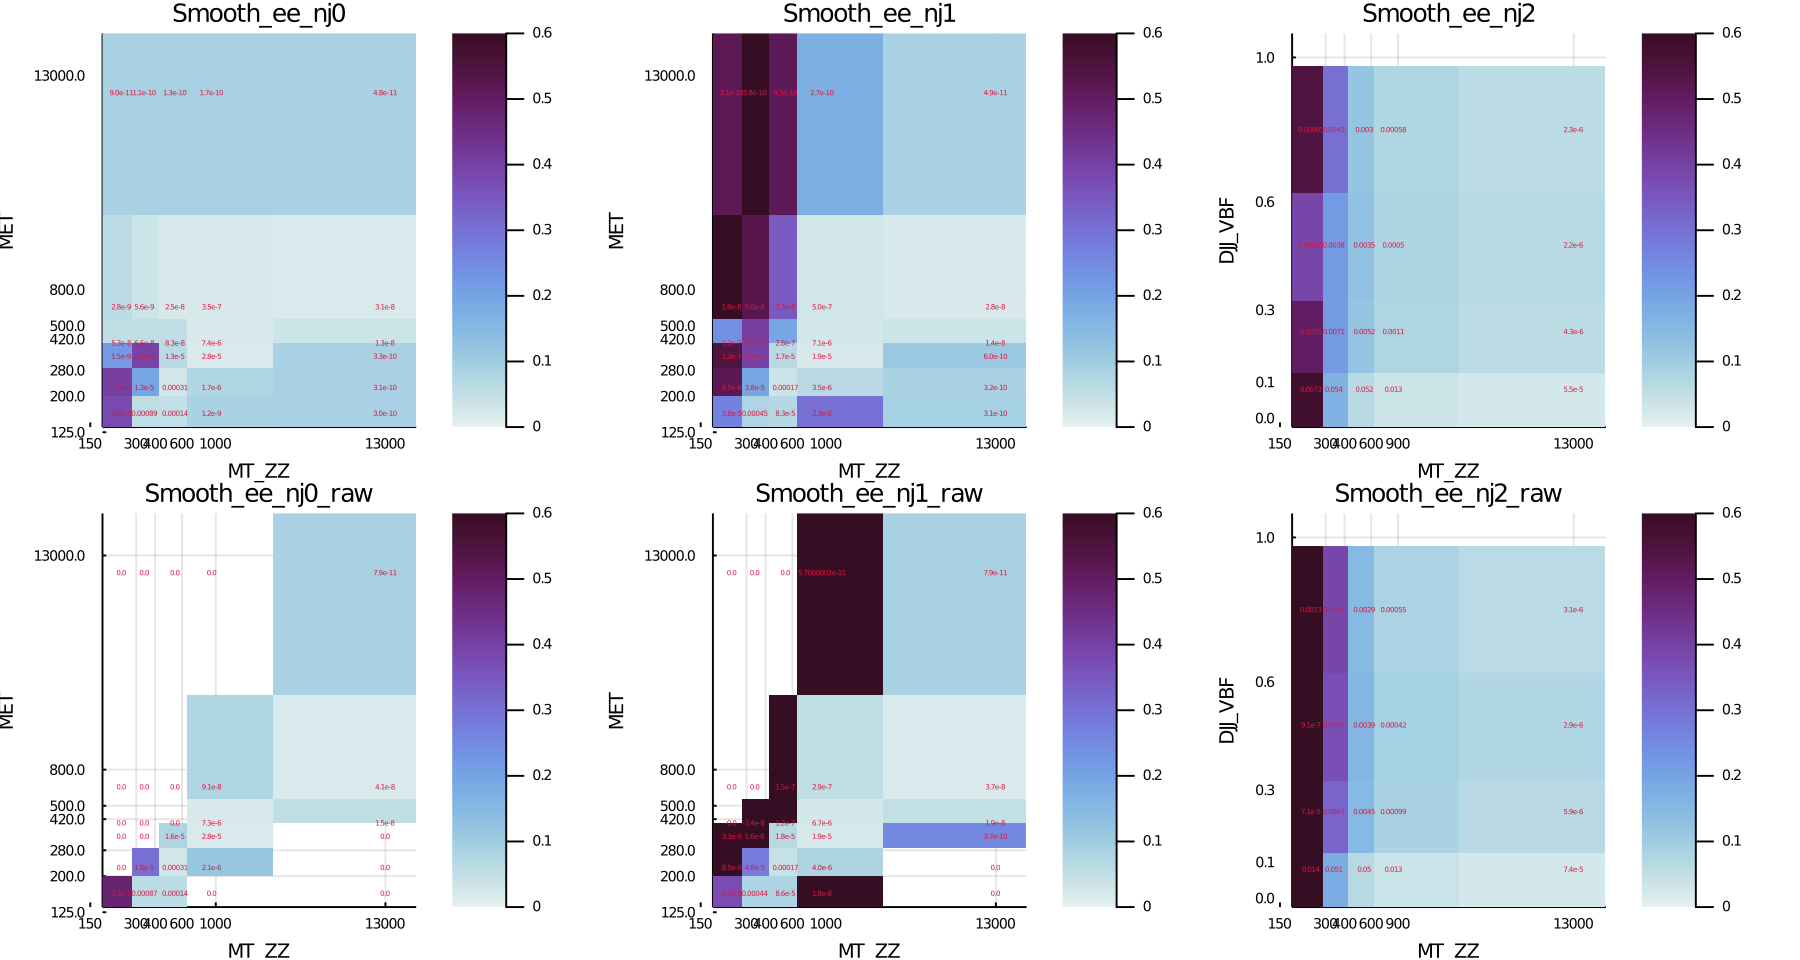
\includegraphics[width=.90\linewidth]{fig/binning_placeholder.png}
\end{center}
\label{fig:sig_rewgt}
\end{figure}
\todo[inline]{make plots publication quality and give quantitative justification for choice}
